\documentclass[11pt]{article}
\usepackage[margin=0.78in]{geometry}
\usepackage{amsmath,amssymb,amsthm,graphicx,microtype}
\usepackage[colorlinks=true,urlcolor=blue,citecolor=blue]{hyperref}

\newtheorem{theorem}{Theorem}
\newtheorem{corollary}{Corollary}
\newcommand{\A}{\mathcal A}
\newcommand{\Ladj}{\mathcal L}
\newcommand{\Kcomp}{\mathcal K}

\title{Submodule preservers on Hilbert modules with\\two orthonormal vectors}
\author{Partial-result packet for \texttt{fa\_banach\_001}\\
\texttt{agent\_lane\_03}, model GPT5.6}
\date{26 August 2026}

\begin{document}
\maketitle

\begin{abstract}
Sharifi asks when an adjointable operator on a Hilbert $C^*$-module that
leaves every closed submodule invariant must be a coefficient morphism, and
poses a compact-operator variant.  We give an exact answer for every right
Hilbert module containing two orthonormal module vectors: the preservers are
precisely right multiplication by central coefficients.  No injectivity,
surjectivity, or nonzero assumption is required.  Consequently the compact
preservers on $\A^n$, $n\geq2$, are exactly the central scalar matrices, while
the only compact preserver on the standard module $\ell^2(\A)$ is zero.  This
is a proved partial answer; arbitrary Hilbert modules without such a pair
remain outside its scope.
\end{abstract}

\section{Source questions and their literal boundary cases}

Sharifi's arXiv:2506.01161 asks in Problem~2.16 (PDF page 11) for which
$C^*$-algebras universal closed-submodule invariance forces an adjointable
operator to equal $I.a$ for a \emph{nonzero} coefficient $a$ \cite{Sharifi}.

\begin{center}
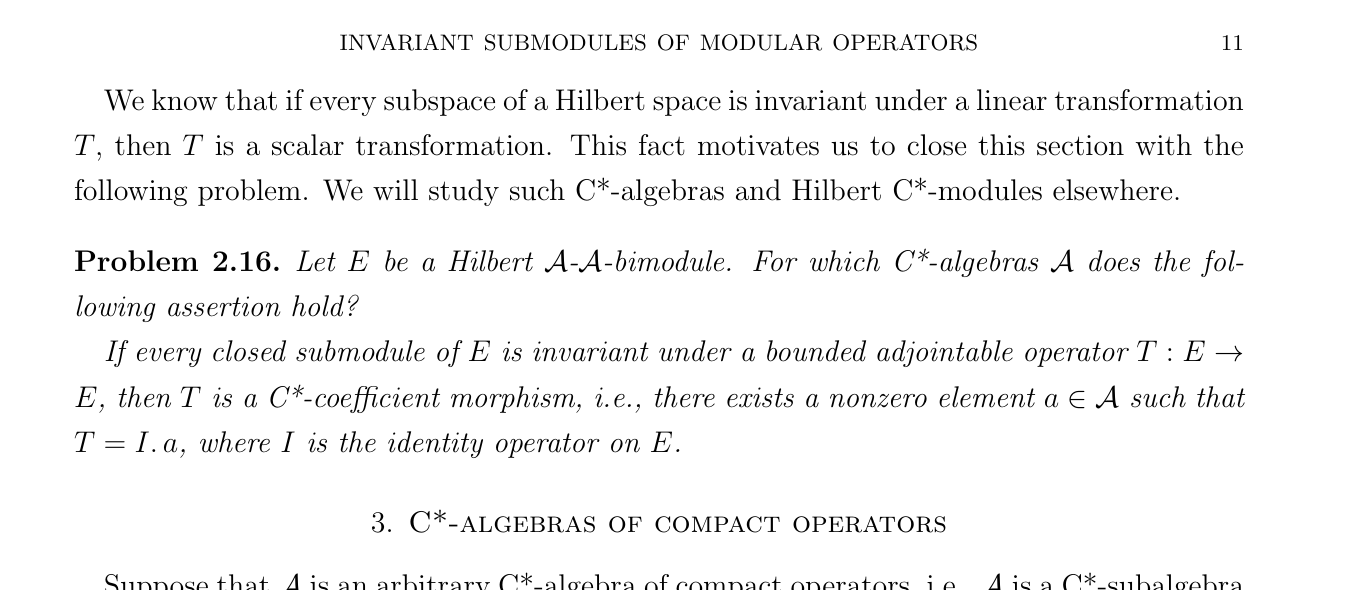
\includegraphics[width=0.96\linewidth]{figures/problem_2_16_crop.png}
\end{center}

Literally, $T=0$ satisfies the hypothesis, but on the faithful standard
module $\A^2$ it cannot equal right multiplication by a nonzero coefficient.
The natural repair is to allow $a=0$, or to assume $T\neq0$.

Problem~4.10 (PDF page 17) asks for the compact analogue under the condition
$I\neq K$.

\begin{center}
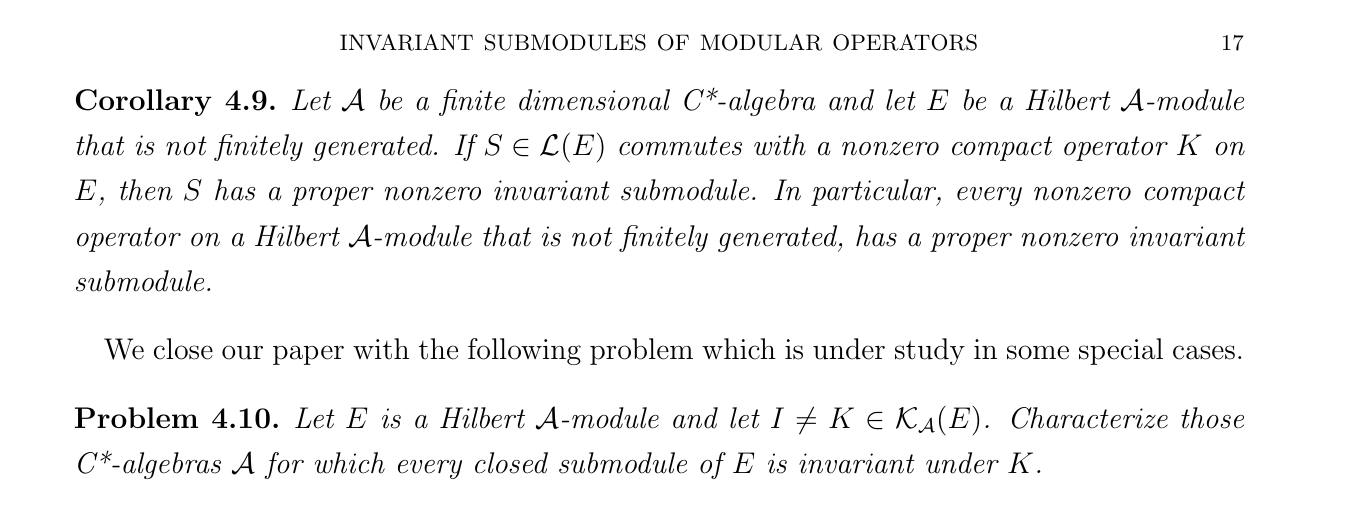
\includegraphics[width=0.96\linewidth]{figures/problem_4_10_crop.png}
\end{center}

That condition still permits $K=0$, which automatically preserves every
submodule.  Below we classify the natural repaired problem on standard and,
more generally, two-orthonormal-vector modules.

\section{Idea of the Proof}

The Hilbert-space proof tests one-dimensional spans.  Here the replacement is
a family of closed cyclic graph submodules.  The coordinate submodules
$e_1\A,e_2\A$ first diagonalize the operator.  The diagonal graph
$(e_1+e_2)\A$ equates the two diagonal coefficients.  The graphs
$(e_1+e_2c)\A$, for arbitrary $c\in\A$, force that common coefficient to
commute with all of $\A$.  Finally, $(e_1+y)\A$ propagates the same
coefficient to the orthogonal complement.  Unlike the known general theorem
for bijective preservers, this argument uses no injectivity at all.

\section{Exact preserver theorem}

Let $\A$ be a unital $C^*$-algebra and $E$ a right Hilbert $\A$-module.  We
use the convention that the inner product is linear in the second variable.
For $z\in Z(\A)$, let $R_z(x)=xz$.

\begin{theorem}\label{thm:main}
Suppose $E$ contains vectors $e_1,e_2$ with
\[
 \langle e_i,e_j\rangle=\delta_{ij}1_{\A}.
\]
For $T\in\Ladj(E)$, the following are equivalent:
\begin{enumerate}
 \item every closed right $\A$-submodule of $E$ is $T$-invariant;
 \item $T=R_z$ for a unique $z\in Z(\A)$.
\end{enumerate}
\end{theorem}

\begin{proof}
Assume (1).  The coordinate submodules $e_i\A$ are closed, so
\[
 T e_1=e_1b_1,\qquad T e_2=e_2b_2
\]
for unique $b_1,b_2\in\A$.  The cyclic submodule
$(e_1+e_2)\A$ is closed and invariant.  Hence
$e_1b_1+e_2b_2=(e_1+e_2)b$ for some $b\in\A$; taking inner products with
$e_1,e_2$ gives $b_1=b_2=b$.

For any $c\in\A$, the map
\[
 a\longmapsto(e_1+e_2c)a
\]
is bounded below, since
\[
 \langle e_1+e_2c,e_1+e_2c\rangle=1+c^*c\geq1.
\]
Its range $W_c=(e_1+e_2c)\A$ is therefore closed.  Invariance gives
\[
 e_1b+e_2bc=T(e_1+e_2c)=(e_1+e_2c)a_c.
\]
The first coordinate yields $a_c=b$, and the second yields $bc=cb$.
As $c$ was arbitrary, $b\in Z(\A)$.

Let $M=e_1\A\oplus e_2\A$ and $F=M^\perp$.  The finite orthonormal
summand $M$ is complemented, so $E=M\oplus F$.  Since $F$ is a closed
submodule, $T(F)\subseteq F$.  For $y\in F$, the same lower-bound argument
shows that $W_y=(e_1+y)\A$ is closed.  Thus
\[
 e_1b+Ty=T(e_1+y)=(e_1+y)a_y.
\]
Uniqueness in $e_1\A\oplus F$ gives $a_y=b$ and $Ty=yb$.  Right
$\A$-linearity and centrality of $b$ now show $Tx=xb$ for every
$x\in E$.  Thus $T=R_b$.

Conversely, if $z\in Z(\A)$, then $R_z$ is adjointable and right
$\A$-linear, with adjoint $R_{z^*}$.  Every right submodule is closed under
right multiplication by $z$, so it is $R_z$-invariant.  Uniqueness follows
from $e_1z=R_z(e_1)$.
\end{proof}

\section{Finite-free and standard-module consequences}

\begin{corollary}\label{cor:standard}
Let $\A$ be a nonzero unital $C^*$-algebra.
\begin{enumerate}
 \item For $2\leq n<\infty$, the operators in $\Ladj(\A^n)=M_n(\A)$
 leaving every closed submodule invariant are exactly $zI_n$ with
 $z\in Z(\A)$.  Since $\Kcomp_{\A}(\A^n)=M_n(\A)$, this is also the exact
 compact classification.
 \item On the standard module $H_{\A}=\ell^2(\A)$, the only
 $K\in\Kcomp_{\A}(H_{\A})$ leaving every closed submodule invariant is
 $K=0$.
 \item The universal-over-all-$E,K$ reading of Problem~4.10 fails for every
 such $\A$: on $E=\A^2$, the compact projection
 $K=\operatorname{diag}(1,0)\neq I$ does not preserve
 $(e_1+e_2)\A$.
\end{enumerate}
\end{corollary}

\begin{proof}
The first assertion is Theorem~\ref{thm:main}.  For the second, that theorem
gives $K=R_z$ with $z\in Z(\A)$.  If $(e_m)$ is the standard orthonormal
sequence, then $\|R_ze_m\|=\|z\|$ for every $m$.  On the other hand,
$\|Fe_m\|\to0$ for every $F\in\Kcomp_{\A}(H_{\A})$: this is immediate for
finite sums of rank-one operators because the coordinates of every vector in
$\ell^2(\A)$ tend to zero, and follows for compact operators by norm
approximation.  Therefore $z=0$.  Finally,
$K(e_1+e_2)=e_1\notin(e_1+e_2)\A$, proving (3).
\end{proof}

\section{Relation to the later partial answer}

Frank's arXiv:2507.11206 explicitly cites Sharifi's Problem~2.16 and proves
that on an arbitrary full Hilbert module every \emph{bijective} bounded module
morphism preserving all norm-closed submodules is multiplication by an
invertible central multiplier \cite[Thm.~1.2]{Frank}.  Frank also states that
a complete result for merely injective preservers is out of reach.  Theorem
\ref{thm:main} is complementary: it permits arbitrary noninjective operators,
but assumes that the module contains two orthonormal vectors.  General modules
without such a pair remain open here.

\section*{Verification, novelty scope, and review recommendation}

The exact script \texttt{code/check\_matrix\_models.py} verifies for
$M_d(\mathbb Q)$, $1\leq d\leq7$, that commutation with all matrix units has
one-dimensional solution space, and checks the diagonal-projection witness.
The proof itself has no computational dependency.

The four local run indexes and current arXiv searches were checked using both
arXiv ids, the exact problem text, ``C*-submodule preserving'', ``Alg Lat'',
central multipliers, orthonormal module vectors, and non-bijective variants.
They found Frank's bijective theorem but no statement matching
Theorem~\ref{thm:main} or Corollary~\ref{cor:standard}.  This is bounded
novelty evidence, not a publication-novelty guarantee.  Human review should
focus on closedness of the graph submodules, the orthogonal-complement step,
and the compactness argument on $\ell^2(\A)$.

\begin{thebibliography}{9}
\bibitem{Sharifi}
K.~Sharifi,
\emph{Invariant submodules of modular operators and Lomonosov type theorem
for Hilbert $C^*$-modules}, arXiv:2506.01161,
\url{https://arxiv.org/abs/2506.01161}.

\bibitem{Frank}
M.~Frank,
\emph{$C^*$-submodule preserving module mappings on Hilbert $C^*$-modules},
arXiv:2507.11206,
\url{https://arxiv.org/abs/2507.11206}.
\end{thebibliography}

\end{document}
